\newcommand{\texname}{2PeriodLCModel}
% Add the listed directories to the search path
% (allows easy moving of files around later)
% these paths are searched AFTER local config kpsewhich

% *.sty, *.cls
\makeatletter
\def\input@path{{@resources/texlive/texmf-local/tex/latex/}
        ,{@resources/texlive/texmf-local/bibtex/bst/},
        ,{@resources/texlive/texmf-local/bibtex/bib/},
        ,{@local/}
        }
\makeatother
\makeatletter
\def\bibinput@path{{@resources/texlive/texmf-local/tex/latex/}
        ,{@resources/texlive/texmf-local/bibtex/bst/},
        ,{@resources/texlive/texmf-local/bibtex/bib/},
        ,{@local/}
        }
\makeatother

\documentclass{scrartcl}
\usepackage{econark-ark-required}\usepackage{econark-multibib,llorracc-handouts,graphicx,hyperref}\usepackage[authoryear]{natbib}
\begin{document}
\handoutHeader

{\centerline {\LARGE The Fisher Two-Period Optimal Consumption Problem }}\vspace{0.15in}



  Irving \cite{fisherInterestTheory} first analyzed the optimization
  problem of a consumer who faces no uncertainty and lives for two
  periods.

  \section{Mathematical Analysis}

  In its most general form, the household's lifetime value function can be written
  \[
    \mathrm{V}(\boldsymbol{\mathit{c}}_{1},\boldsymbol{\mathit{c}}_{2})
  \]
  where the first argument reflects consumption in `youth' while the second argument represents consumption in `old age' and we assume that the derivatives with respect to the first and second arguments are positive,
  \begin{equation}
    \mathrm{V}_{1}, \mathrm{V}_{2} > 0, \label{eq:uprimepos}
  \end{equation}
  while the second derivatives are negative,
  \begin{equation}
    \mathrm{V}_{11}, \mathrm{V}_{22}<0 \label{eq:uprimeprimeneg}.
  \end{equation}

  The consumer begins the first period with resources of $\boldsymbol{\mathit{b}}_{1}$ (think `bank balances') and income of $\boldsymbol{\mathit{y}}_{1}$.
  Total resources are divided between consumption and end-of-period assets $\boldsymbol{\mathit{a}}_{1}$ (`assets after all actions' in period ${1}$):
  \begin{equation}\begin{gathered}\begin{aligned}
        \boldsymbol{\mathit{b}}_{1}+\boldsymbol{\mathit{y}}_{1} & =  \boldsymbol{\mathit{c}}_{1}+\boldsymbol{\mathit{a}}_{1},
        \\ \boldsymbol{\mathit{a}}_{1} & =  \boldsymbol{\mathit{b}}_{1}+\boldsymbol{\mathit{y}}_{1}-\boldsymbol{\mathit{c}}_{1}.
      \end{aligned}\end{gathered}\end{equation}

  Balances at the beginning of period 2 are equal to end-of-first-period accumulated assets $\boldsymbol{\mathit{a}}_{1}$, rewarded by a gross interest factor $\mathsf{R} = (1+\mathsf{r})$:
  \begin{equation}\begin{gathered}\begin{aligned}
        \boldsymbol{\mathit{b}}_{2} & =  \boldsymbol{\mathit{a}}_{1}\mathsf{R}.
      \end{aligned}\end{gathered}\end{equation}

  This is the \textit{dynamic budget constraint} or DBC for this problem.
  A DBC links two adjacent periods of time.
  A more comprehensive kind of constraint is the \textit{intertemporal} budget constraint (IBC):
  \begin{equation}\begin{gathered}\begin{aligned} \boldsymbol{\mathit{c}}_{1}+\boldsymbol{\mathit{c}}_{2}/\mathsf{R} & \leq \boldsymbol{\mathit{y}}_{1}+\boldsymbol{\mathit{y}}_{2}/\mathsf{R}+\boldsymbol{\mathit{b}}_{1} \label{eq:ibcineq},
      \end{aligned}\end{gathered}\end{equation} which must be satisfied over an extended (multiperiod) span of time like a lifetime.

  For various purposes, it is useful to keep track of \textit{human wealth} $\boldsymbol{\mathit{h}}_{t}$, defined as the present discounted value of future labor income (the operator ${\mathbb{P}}_{t}(\bullet)$ denotes the present discounted value of the variable $\bullet$ from the perspective of the beginning of period $t$ through the end of the horizon),
  \begin{equation}\begin{gathered}\begin{aligned} \boldsymbol{\mathit{h}}_{t} & = {\mathbb{P}}_{t}(y) \label{eq:humw} \\ \boldsymbol{\mathit{h}}_{1} & = \boldsymbol{\mathit{y}}_{1}+\boldsymbol{\mathit{y}}_{2}/\mathsf{R}
      \end{aligned}\end{gathered}\end{equation}

  Because we have assumed (in \eqref{eq:uprimepos}) that an additional unit of consumption always yields extra utility, we can reach our first conclusion (as opposed to assumption) in the model: Once the consumer has reached the last period of life, he will consume all available resources:
  \begin{equation}\begin{gathered}\begin{aligned} \boldsymbol{\mathit{c}}_{2} & = \boldsymbol{\mathit{b}}_{2}+\boldsymbol{\mathit{y}}_{2}.
      \end{aligned}\end{gathered}\end{equation}

  This means that the IBC will hold with equality (if it did not, utility could be increased by consuming more in one or both periods).
  Thus, the IBC can be rewritten as
  \begin{equation}\begin{gathered}\begin{aligned} \boldsymbol{\mathit{c}}_{1}+\boldsymbol{\mathit{c}}_{2}/\mathsf{R} & = \boldsymbol{\mathit{h}}_{1}+\boldsymbol{\mathit{b}}_{1} \label{eq:ibc}.
      \end{aligned}\end{gathered}\end{equation}

  The general form that the IBC will take is that the present discounted value of lifetime spending must equal the present discounted value of lifetime resources:
  \begin{equation}\begin{gathered}\begin{aligned} {\mathbb{P}}_{t}(\boldsymbol{\mathit{c}}) & = {\mathbb{P}}_{t}(y)+\boldsymbol{\mathit{b}}_{t}. \label{eq:ibcgen}
      \end{aligned}\end{gathered}\end{equation}

  Substituting in the definition of $\boldsymbol{\mathit{b}}_{2}$ means that our problem can now be stated as:
  \begin{equation}\begin{gathered}\begin{aligned} \max_{\{\boldsymbol{\mathit{c}}_{1},\boldsymbol{\mathit{c}}_{2}\}} & \mathrm{V}(\boldsymbol{\mathit{c}}_{1},\boldsymbol{\mathit{c}}_{2}) \\ & \mbox{s.t.}  \nonumber \\ \boldsymbol{\mathit{c}}_{2} & = (\boldsymbol{\mathit{b}}_{1}+\boldsymbol{\mathit{y}}_{1}-\boldsymbol{\mathit{c}}_{1})\mathsf{R}+\boldsymbol{\mathit{y}}_{2}.
      \end{aligned}\end{gathered}\end{equation}

  Now we can write the problem as a \href{https://en.wikipedia.org/wiki/Lagrange_multiplier}{Lagrange multiplier} problem, where the maximand is:
  \begin{equation} \mathrm{V}(\boldsymbol{\mathit{c}}_{1},\boldsymbol{\mathit{c}}_{2}) + \left( \boldsymbol{\mathit{c}}_{2}- (\boldsymbol{\mathit{b}}_{1}+\boldsymbol{\mathit{y}}_{1}-\boldsymbol{\mathit{c}}_{1})\mathsf{R}-\boldsymbol{\mathit{y}}_{2}\right)\lambda.
  \end{equation}

  The first order conditions are:
  \begin{equation}\begin{gathered}\begin{aligned} \mathrm{V}_{1} + \mathsf{R}\lambda & = 0 \label{eq:lagrange1} \\ \mathrm{V}_{2} & = -\lambda
      \end{aligned}\end{gathered}\end{equation} and substituting the second of these into the first we get
  \begin{equation}\begin{gathered}\begin{aligned} \mathrm{V}_{1} & = \mathsf{R} \mathrm{V}_{2} \label{eq:timeprice}.
      \end{aligned}\end{gathered}\end{equation}

  This is the same condition you get when deciding between two commodities at a point in time, where we can now think of $\mathsf{R}$ as the intertemporal price: How much of good 2 (consumption in period 2) do I get in exchange for giving up a unit of good 1 (consumption in period 1).

  Now suppose that the consumer's utility is \textit{time-separable}, and the felicity function (felicity is the utility obtained in a single period of a multi-period problem) is the same in both periods of life, so that
  \begin{equation}\begin{gathered}\begin{aligned} \mathrm{V}(\boldsymbol{\mathit{c}}_{1},\boldsymbol{\mathit{c}}_{2}) & = \mathrm{u}(\boldsymbol{\mathit{c}}_{1})+\beta \mathrm{u}(\boldsymbol{\mathit{c}}_{2})
      \end{aligned}\end{gathered}\end{equation} where $\beta$ is a \textit{time preference factor} that specifies how the consumer trades off utility in period 1 against utility in period 2.\footnote{Paul~\cite{samuelson1937note,samuelsonOLG} introduced the discounting of future utility into the problem.
    See~\cite{floDiscounting} for a comprehensive review of the still-controversial topic of time discounting.}

  From our assumptions \eqref{eq:uprimepos} and \eqref{eq:uprimeprimeneg} we know that the felicity function must satisfy
  \begin{equation}\begin{gathered}\begin{aligned} \mathrm{u}^{\prime}(\bullet) & > 0 \\ \mathrm{u}^{\prime\prime}(\bullet) & < 0,
      \end{aligned}\end{gathered}\end{equation} and since the felicity functions are the same in both periods we have that
  \begin{equation}\begin{gathered}\begin{aligned} \mathrm{V}_{1}(\boldsymbol{\mathit{c}}_{1},\boldsymbol{\mathit{c}}_{2}) & = \mathrm{u}^{\prime}(\boldsymbol{\mathit{c}}_{1}) \\ \mathrm{V}_{2}(\boldsymbol{\mathit{c}}_{1},\boldsymbol{\mathit{c}}_{2}) & = \beta \mathrm{u}^{\prime}(\boldsymbol{\mathit{c}}_{2}).
      \end{aligned}\end{gathered}\end{equation}

  Substituting these equations into \eqref{eq:timeprice} yields the \textit{Euler equation} for consumption:
  \begin{equation}\begin{gathered}\begin{aligned} \mathrm{u}^{\prime}(\boldsymbol{\mathit{c}}_{1}) & = \mathsf{R} \beta \mathrm{u}^{\prime}(\boldsymbol{\mathit{c}}_{2}). \label{eq:euler}
      \end{aligned}\end{gathered}\end{equation}

  The Euler equation is a central result in intertemporal optimization theory, and will be used again and again as the course progresses.
  It is therefore worth studying carefully to be sure you understand it thoroughly.

  To help obtain the intuition for why the Euler equation is necessary for optimality, consider the following thought experiment.
  Designate $\boldsymbol{\mathit{c}}^{*}_{1}$ and $\boldsymbol{\mathit{c}}^{*}_{2}$ as the optimal levels of consumption in this problem, the levels that solve the maximization problem under some set of circumstances.
  Thus, the highest attainable utility is
  \begin{equation} \mathrm{u}(\boldsymbol{\mathit{c}}_{1}^{*})+\beta \mathrm{u}(\boldsymbol{\mathit{c}}_{2}^{*}) \label{eq:maxutil}.
  \end{equation}

  Now consider reducing consumption by some small amount $\epsilon$ in period 1, investing that $\epsilon$ so that it grows to $\mathsf{R} \epsilon$ in period 2, and then consuming it in period 2.
  What happens to utility?

  Taking first-order Taylor expansions, the levels of first-period and second-period utility are now
  \begin{equation}\begin{gathered}\begin{aligned} \mathrm{u}(\boldsymbol{\mathit{c}}_{1}^{*}-\epsilon) & \approx \mathrm{u}(\boldsymbol{\mathit{c}}_{1}^{*})-\mathrm{u}^{\prime}(\boldsymbol{\mathit{c}}_{1}^{*})\epsilon \\ \mathrm{u}(\boldsymbol{\mathit{c}}_{2}^{*}+\mathsf{R}\epsilon) & \approx \mathrm{u}(\boldsymbol{\mathit{c}}_{2}^{*})+\mathrm{u}^{\prime}(\boldsymbol{\mathit{c}}_{2}^{*})\mathsf{R}\epsilon.
      \end{aligned}\end{gathered}\end{equation}

  Now the difference between the maximum possible utility and the new situation is given by
  \begin{equation} \mathrm{u}(\boldsymbol{\mathit{c}}_{1}^{*})+\beta \mathrm{u}(\boldsymbol{\mathit{c}}_{2}^{*}) - \left[\mathrm{u}(\boldsymbol{\mathit{c}}_{1}^{*})-\mathrm{u}^{\prime}(\boldsymbol{\mathit{c}}_{1}^{*})\epsilon + \beta \left(\mathrm{u}(\boldsymbol{\mathit{c}}_{2}^{*})+\mathrm{u}^{\prime}(\boldsymbol{\mathit{c}}_{2}^{*})\mathsf{R}\epsilon \right) \right] = \mathrm{u}^{\prime}(\boldsymbol{\mathit{c}}_{1}^{*})\epsilon - \beta \mathrm{u}^{\prime}(\boldsymbol{\mathit{c}}_{2}^{*})\mathsf{R}\epsilon \label{eq:diffutil}.
  \end{equation}

  But it must be the case that \eqref{eq:diffutil} is approximately equal to zero.
  To see why, suppose it were a negative number.
  That would mean that moving from the original situation with $\{\boldsymbol{\mathit{c}}_{1},\boldsymbol{\mathit{c}}_{2}\} = \{\boldsymbol{\mathit{c}}_{1}^{*},\boldsymbol{\mathit{c}}_{2}^{*}\}$ to the new situation with $\{\boldsymbol{\mathit{c}}_{1},\boldsymbol{\mathit{c}}_{2}\} = \{\boldsymbol{\mathit{c}}_{1}^{*}-\epsilon,\boldsymbol{\mathit{c}}_{2}^{*}+\mathsf{R}\epsilon\}$ resulted in an \textit{ increase} in utility.
  But we assumed that $\boldsymbol{\mathit{c}}_{1}^{*},\boldsymbol{\mathit{c}}_{2}^{*}$ were already the utility-maximizing choices, which clearly could not be true if adjusting $\boldsymbol{\mathit{c}}_{1}^{*}$ downward by $\epsilon$ and $\boldsymbol{\mathit{c}}^{*}_{2}$ upward by $\mathsf{R} \epsilon$ increased utility.
  Similarly, if the expression were positive, then utility could be increased by doing the opposite (i.e.\ increasing consumption in period 1 by $\epsilon$ and reducing it in period 2 by $\mathsf{R}\epsilon$).
  Thus, in either case if the expression is not zero, we have a contradiction to the assumption that $\boldsymbol{\mathit{c}}_{1}^{*}$ and $\boldsymbol{\mathit{c}}_{2}^{*}$ are the utility-maximizing choices.

  To make further progress, it is necessary to make more specific assumptions about the structure of the utility function.
  The most common assumption is that utility takes the Constant Relative Risk Aversion form,
  \begin{equation}\begin{gathered}\begin{aligned} \mathrm{u}(\boldsymbol{\mathit{c}}) & = \left(\frac{\boldsymbol{\mathit{c}}^{1-\rho}}{1-\rho}\right) \label{eq:crrautil},
      \end{aligned}\end{gathered}\end{equation} with marginal utility
  \begin{equation}\begin{gathered}\begin{aligned} \mathrm{u}^{\prime}(\boldsymbol{\mathit{c}}) & = \boldsymbol{\mathit{c}}^{-\rho} \label{eq:crramargutil}.
      \end{aligned}\end{gathered}\end{equation}

  Consider equation \eqref{eq:euler} with CRRA utility,
  \begin{equation}\begin{gathered}\begin{aligned} \boldsymbol{\mathit{c}}_{1}^{-\rho} & = \mathsf{R}\beta \boldsymbol{\mathit{c}}_{2}^{-\rho} \\ \boldsymbol{\mathit{c}}_{2}/\boldsymbol{\mathit{c}}_{1} & = (\mathsf{R}\beta)^{1/\rho} \\ \boldsymbol{\mathit{c}}_{2} & = (\mathsf{R}\beta)^{1/\rho}\boldsymbol{\mathit{c}}_{1} \label{eq:c1euler}.
      \end{aligned}\end{gathered}\end{equation}

  Now note that this equation allows us to calculate the \textit{intertemporal elasticity of substitution} as the change in the ratio of the log of $\boldsymbol{\mathit{c}}_{2}/\boldsymbol{\mathit{c}}_{1}$ to the log change in the intertemporal price $\mathsf{R}$:
  \begin{equation}\begin{gathered}\begin{aligned} \left(\frac{d}{d \log \mathsf{R}}\right) \log \left(\frac{\boldsymbol{\mathit{c}}_{2}}{\boldsymbol{\mathit{c}}_{1}}\right) & = \left(\frac{d}{d \log \mathsf{R}}\right) \log (\mathsf{R} \beta)^{1/\rho} \\ & = \rho^{-1}.
      \end{aligned}\end{gathered}\end{equation}

  Next note that from \eqref{eq:c1euler} we can calculate the PDV of lifetime consumption from the perspective of the first period of life as
  \begin{equation}\begin{gathered}\begin{aligned} {\mathbb{P}}_{1}(\boldsymbol{\mathit{c}}) & = \boldsymbol{\mathit{c}}_{1} + \mathsf{R}^{-1}\boldsymbol{\mathit{c}}_{2} \\ & = \left(1+\mathsf{R}^{-1}(\mathsf{R}\beta)^{1/\rho}\right)\boldsymbol{\mathit{c}}_{1}.
      \end{aligned}\end{gathered}\end{equation}

  Now we can use the intertemporal budget constraint:
  \begin{equation}\begin{gathered}\begin{aligned} {\mathbb{P}}_{t}(\boldsymbol{\mathit{c}}) & = \boldsymbol{\mathit{b}}_{t}+{\mathbb{P}}_{t}(y) \\ \boldsymbol{\mathit{c}}_{1}\left(1+\mathsf{R}^{-1}(\mathsf{R}\beta)^{1/\rho}\right) & = \boldsymbol{\mathit{b}}_{1}+\boldsymbol{\mathit{y}}_{1}+\mathsf{R}^{-1}\boldsymbol{\mathit{y}}_{2} \\ \boldsymbol{\mathit{c}}_{1} & = \left(\frac{\boldsymbol{\mathit{b}}_{1}+\boldsymbol{\mathit{h}}_{1}}{1+\mathsf{R}^{-1}(\mathsf{R}\beta)^{1/\rho}}\right).
      \end{aligned}\end{gathered}\end{equation}

  Thus, we have solved the two-period life cycle saving problem for the \textit{consumption function} $\mathrm{c}_{1}$ relating the level of consumption to all of the parameters of the problem.

  One of the surprising features of the solution goes by the name of ``Fisherian Separation'': Notice that the \textit{profile} of consumption growth over the lifetime is given by \eqref{eq:c1euler} \textit{regardless of the shape of the income profile}.
  For two consumers with the same total amount of lifetime wealth (combined $\boldsymbol{\mathit{b}}_{1}$ and $\boldsymbol{\mathit{h}}_{1}$, the level and growth rates of consumption over the lifetime will be identical whether the consumer's lifetime wealth is entirely concentrated in the first period (that is, $\boldsymbol{\mathit{h}}_{1}=0$), entirely concentrated in the last period ($\boldsymbol{\mathit{b}}_{1}=0$), split half-and-half, or organized any other way.
  Fisherian Separation is a pervasive feature of models that combine perfect foresight and a lack of liquidity constraints.

  A common assumption (for simplicity, not realism) is that $\rho=1$, which is equivalent to assuming that the utility function is logarithmic:\footnote{See math fact \CRRALim in \MathFactsList.}
  \begin{equation}\begin{gathered}\begin{aligned} \lim_{\rho \rightarrow 1} \left(\frac{\boldsymbol{\mathit{c}}^{1-\rho}}{1-\rho}\right) & = \log c.
      \end{aligned}\end{gathered}\end{equation}

  In this case it turns out that we can simply substitute $\rho=1$ into the solution for consumption, obtaining
  \begin{equation}\begin{gathered}\begin{aligned} \mathrm{c}_{1} & = \left(\frac{\boldsymbol{\mathit{b}}_{1}+\boldsymbol{\mathit{h}}_{1}}{1+\beta}\right).
      \end{aligned}\end{gathered}\end{equation}


  \section{Graphical Analysis}

  The classic graphical analysis of this problem is shown in figure \ref{fig:Fisher}.

  The top figure depicts a situation in which all of the consumer's lifetime income is earned in the first period of life.
  The budget constraint in the initial situation, associated with a ``Low $\mathsf{R}$'', yields an optimal consumption choice labeled as point $A$ where the budget constraint is tangent to the indifference curve.
  When the interest factor is increased to the ``High $\mathsf{R}$'' situation, the optimal consumption choice moves to point $C$.

  Note first that if all income is earned in the first period of life, an increase in the interest factor is unambiguously good for the consumer - the set of consumption possibilities is strictly larger.

  Second, the movement from point $A$ to point $C$ can be decomposed into two parts: an income effect $AB$ and a substitution effect $BC$.

  Call the low and the high interest factors respectively $\underline{\mathsf{R}}$ and $\bar{\mathsf{R}}$.

  The income effect is the answer to the question ``Suppose we wanted to change lifetime value by the same amount as it is changed by going from $\underline{\mathsf{R}}$ to $\bar{\mathsf{R}}$, but we wanted to achieve this change in value at the initial interest factor $\underline{\mathsf{R}}$.
  Supposing we gave the consumer enough extra initial resources to achieve the change in value, how would their consumption allocation change?''

  In order to relate this back to the algebraic analysis above, it will be useful to rewrite lifetime value as a function simply of initial resources and the interest factor (taking ${\boldsymbol{\mathit{y}}_{1},\boldsymbol{\mathit{y}}_{2}}$ and other parts of the problem as given):
  \begin{equation}\begin{gathered}\begin{aligned} \mathrm{V}^{*}(\boldsymbol{\mathit{b}}_{1},\mathsf{R}) & = \mathrm{u}(\mathrm{c}_{1}^{*}(\boldsymbol{\mathit{b}}_{1},\mathsf{R}))+\beta \mathrm{u}(\mathrm{c}_{2}^{*}(\boldsymbol{\mathit{b}}_{1},\mathsf{R}))
      \end{aligned}\end{gathered}\end{equation}

  Using this function, the income effect is obtained as the value of $\Delta \boldsymbol{\mathit{b}}_{1}$ in the equation $\mathrm{V}^{*}(\boldsymbol{\mathit{b}}_{1}+\Delta \boldsymbol{\mathit{b}}_{1},\underline{\mathsf{R}})=\mathrm{V}^{*}(\boldsymbol{\mathit{b}}_{1},\bar{\mathsf{R}})$.

  The substitution effect is the answer to the question, ``Staying on the new indifference curve, how much does the allocation of consumption change as a consequence of the difference in interest factors between $\underline{\mathsf{R}}$ and $\bar{\mathsf{R}}$?''  This is captured in the movement from $B$ to $C$.

  Note that the income and the substitution effects on $\boldsymbol{\mathit{c}}_{1}$ are opposite in sign.
  A higher interest factor gives consumers the incentive to substitute future for current consumption ($\boldsymbol{\mathit{c}}_{1}$ is lower at point $C$ than at $B$).
  But a higher interest factor also gives consumers the ability to consume more in both periods.
  Whether $\boldsymbol{\mathit{c}}_{1}$ rises or falls in response to the increase in interest factors will depend on the relative magnitudes of the income and substitution effects.

  The lower figure shows a similar experiment, with the sole difference that the consumer's lifetime resources are exclusively concentrated in period 2.

  In this case, the period 1 consumer must borrow against future income in order to consume anything.
  An increase in interest factors is therefore unambiguously bad (the available set of consumption choices is strictly smaller).

  The optimal choice again moves from point $A$ to point $C$.
  However, we now decompose the movement into three parts.
  The first part is called the \textit{human wealth effect}.
  It captures the fact that the present discounted value of lifetime resources ${\mathbb{P}}_{1}(y)$ is smaller when interest rates are higher; the magnitude of the change in human wealth is depicted on the horizontal axis of the figure.
  The human wealth \textit{effect} is the consequence that an equivalent change in lifetime resources would have \textit{in the absence of any change in interest factors}.
  So the human wealth effect takes the consumer from point $A$ to point $D$.

  Notice that once we have computed the human wealth effect, if we treat point $D$ as the starting point of our analysis, the remaining analysis is identical to that for the upper figure: We can increase the interest factor from $\underline{\mathsf{R}}$ to $\bar{\mathsf{R}}$, which causes the equilibrium point to change from point $D$ to point $C$, a movement that can be decomposed into an income effect $DB$ (analogous to the income effect $AB$ in the original analysis) and a substitution effect $BC$.

  The terminology here is a modification (refinement) of the terminology often employed in micro textbooks, where the ``income effect'' is defined in a way that would incorporate both what I am calling the income effect and what I am calling the human wealth effect.

  The reason to make this distinction is that it is important to distinguish between effects on behavior caused by the fact that the discounted value of future income is changed, and effects caused by the fact that the income that will be earned on savings is different.
  \cite{summersCapTax} vigorously made the point that in standard life cycle models, the quantitative magnitude of the human wealth effect dwarfs the size of either the income or the substitution effects, because for most people most of their lifetime income is in the future.

  \begin{figure}
    \caption{Fisher Figure Analysis}\label{fig:Fisher} 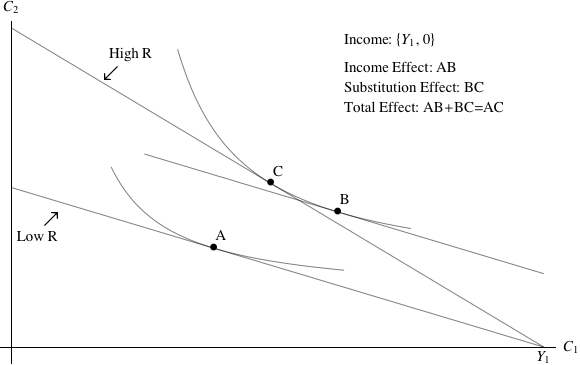
\includegraphics[width=6in]{./Figures/FisherFigureY1} 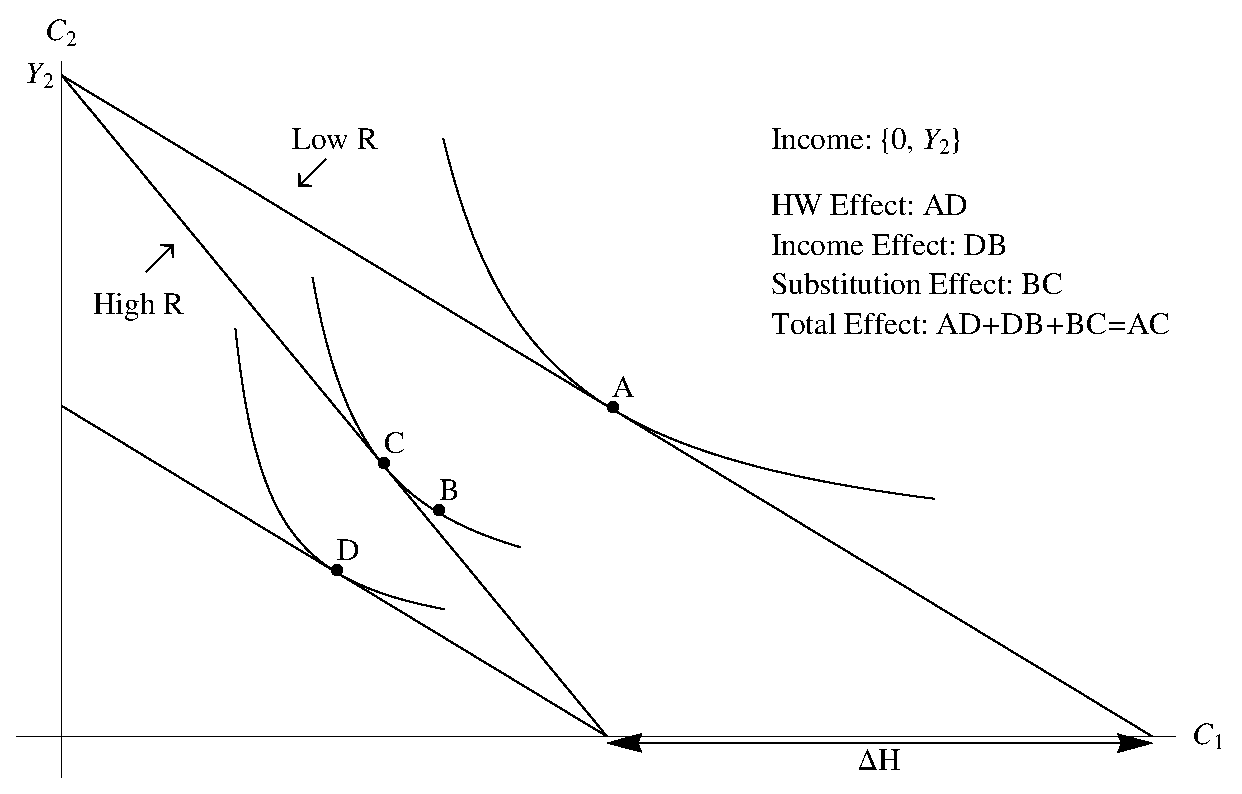
\includegraphics[width=6in]{./Figures/FisherFigureY2}
  \end{figure}


\bibliographystyle{econark}\bibliography{\texname}

\end{document}

